\problemname{Apples and Pears}

Axel wants to compete with Petra about who has sold the most apples and pears, but Petra thinks that one cannot
”compare apples and pears”. 
They agree instead to compare how much money they have earned. They ask you to create a program that,
given the number of apples Axel has sold and the number of pears Petra has sold, prints who has earned
the most (or ”\texttt{lika}” if they have sold for the same amount). Apples cost $7$ kronor each and pears $13$ kronor each.

\begin{center}
  
\includegraphics[width=5cm]{apple.jpg}
  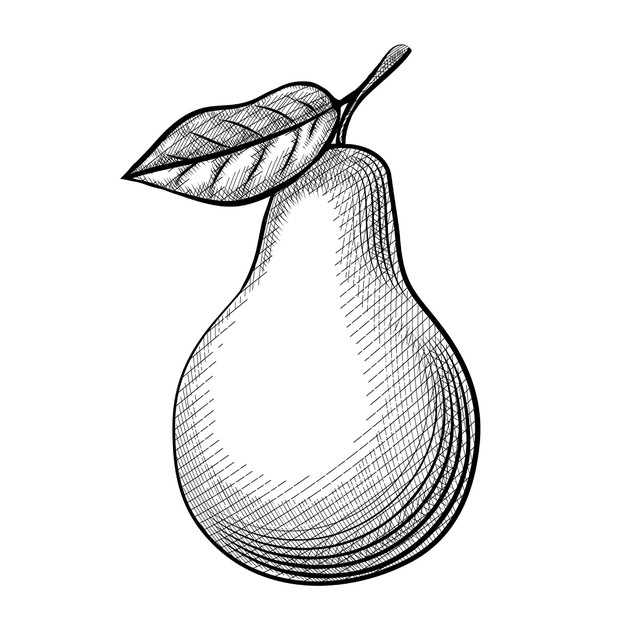
\includegraphics[width=5cm]{pear.jpg}
\end{center}


\section*{Input}
The input consists of a single line with two integers $A,P$ ($0 \leq A,P \leq 1000$),
the number of apples Axel has managed to sell, and the number of pears Petra has managed to sell.

\section*{Output}
Print a string: the person who has earned the most, ”\texttt{Axel}” or ”\texttt{Petra}”.
If they have sold for the same amount, print ”\texttt{lika}”.

\section*{Points}
Your solution will be tested on several test case groups.
To get the points for a group, it must pass all the test cases in the group.

\noindent
\begin{tabular}{| l | l | p{12cm} |}
  \hline
  \textbf{Group} & \textbf{Point value} & \textbf{Constraints} \\ \hline
  $1$   & $40$       & Axel and Petra haven't earned the same amount of money. \\ \hline
  $2$   & $60$       & No additional constraints. \\ \hline
\end{tabular}

